\documentclass[11pt,a4paper]{article}

\usepackage[utf8]{inputenc}
\usepackage[T1]{fontenc}
\usepackage[margin=1in]{geometry}
\usepackage{graphicx}
\usepackage{amsmath}
\usepackage{amsfonts}
\usepackage{amssymb}
\usepackage{booktabs}
\usepackage{float}

\title{Lab 3:Genetic Algorithm for Quadratic Equation Solving}
\date{}

\begin{document}

\maketitle

\section{Introduction}

Genetic Algorithms are evolutionary computational techniques inspired by natural selection and genetics. They belong to the class of evolutionary algorithms and are particularly effective for optimization problems where traditional analytical methods may be insufficient or computationally expensive.

In this lab, we implement a genetic algorithm to solve the quadratic equation:
\begin{equation}
2x^2 + 11x + 12 = 0
\end{equation}

The algorithm uses binary encoding to represent potential solutions and employs selection, crossover, and mutation operations to evolve the population towards optimal solutions.

\section{Body of the Lab}

\subsection{Theory}

The quadratic equation $2x^2 + 11x + 12 = 0$ has analytical solutions:
\begin{align}
x_1 &= \frac{-11 + \sqrt{121 - 96}}{4} = \frac{-11 + 5}{4} = -1.5 \
x_2 &= \frac{-11 - \sqrt{121 - 96}}{4} = \frac{-11 - 5}{4} = -4.0
\end{align}

Our genetic algorithm approach involves:
\begin{itemize}
\item Representing solutions as binary chromosomes
\item Using fitness function $f(x) = \frac{1}{1 + |2x^2 + 11x + 12|}$
\item Applying roulette wheel selection
\item Implementing single-point crossover
\item Using bit-flip mutation
\end{itemize}

\subsection{Implementation Parameters}

Based on the configuration file, the algorithm uses:
\begin{itemize}
\item Binary encoding: 3 bits for integer part, 6 bits for fractional part
\item Population size: 283
\item Mutation probability: 0.25
\item Number of generations: 641
\end{itemize}

\subsection{Code Implementation}

The implementation consists of two main classes:
\begin{itemize}
\item \texttt{GeneticAlgorithm}: Basic implementation for positive solutions
\item \texttt{EnhancedGeneticAlgorithm}: Extended version handling negative solutions
\end{itemize}

\subsubsection{GeneticAlgorithm Class Structure}

The main \texttt{GeneticAlgorithm} class initializes with the following parameters:

\begin{verbatim}
class GeneticAlgorithm:
    def __init__(self, a, b, c, integer_bits=3, fraction_bits=6, 
                 population_size=283, mutation_rate=0.25, generations=641):
        self.a, self.b, self.c = a, b, c
        self.integer_bits = integer_bits
        self.fraction_bits = fraction_bits
        self.chromosome_length = integer_bits + fraction_bits
        self.population_size = population_size
        self.mutation_rate = mutation_rate
        self.generations = generations
\end{verbatim}

\subsubsection{Binary Encoding/Decoding}

The algorithm uses binary representation with separate integer and fractional parts:

\begin{verbatim}
def binary_to_decimal(self, chromosome):
    """Convert binary chromosome to decimal value"""
    integer_part = chromosome[:self.integer_bits]
    fraction_part = chromosome[self.integer_bits:]
    
    # Convert integer part
    integer_value = 0
    for i, bit in enumerate(integer_part):
        integer_value += bit * (2**(self.integer_bits - 1 - i))
    
    # Convert fraction part
    fraction_value = 0
    for i, bit in enumerate(fraction_part):
        fraction_value += bit * (2**(-i-1))
        
    return integer_value + fraction_value
\end{verbatim}

\subsubsection{Fitness Function}

The fitness function evaluates how close a solution is to the actual root:

\begin{verbatim}
def fitness_function(self, x):
    """Calculate fitness for equation ax² + bx + c = 0"""
    error = abs(self.a * x**2 + self.b * x + self.c)
    fitness = 1 / (error + 1e-10)  # Avoid division by zero
    return fitness
\end{verbatim}

\subsubsection{Selection Method}

Roulette wheel selection is implemented with probability proportional to fitness:

\begin{verbatim}
def roulette_wheel_selection(self, population, fitness_scores):
    """Roulette wheel selection implementation"""
    total_fitness = sum(fitness_scores)
    probabilities = [f / total_fitness for f in fitness_scores]
    
    r = random.random()
    cumulative_prob = 0
    for i, prob in enumerate(probabilities):
        cumulative_prob += prob
        if r <= cumulative_prob:
            return population[i]
    return population[-1]
\end{verbatim}

\subsubsection{Crossover Operation}

Single-point crossover creates offspring by combining parent chromosomes:

\begin{verbatim}
def single_point_crossover(self, parent1, parent2):
    """Single point crossover"""
    crossover_point = random.randint(1, len(parent1) - 1)
    offspring1 = parent1[:crossover_point] + parent2[crossover_point:]
    offspring2 = parent2[:crossover_point] + parent1[crossover_point:]
    return offspring1, offspring2
\end{verbatim}

\subsubsection{Mutation Operation}

Bit-flip mutation with probability 0.25:

\begin{verbatim}
def mutate(self, chromosome):
    """Bit flip mutation"""
    mutated = chromosome[:]
    for i in range(len(mutated)):
        if random.random() < self.mutation_rate:
            mutated[i] = 1 - mutated[i]  # Flip bit
    return mutated
\end{verbatim}

\subsubsection{Enhanced Implementation for Negative Roots}

The \texttt{EnhancedGeneticAlgorithm} extends the base class to handle negative values by mapping binary representation to a specified range:

\begin{verbatim}
class EnhancedGeneticAlgorithm(GeneticAlgorithm):
    def __init__(self, a, b, c, integer_bits=3, fraction_bits=6, 
                 population_size=283, mutation_rate=0.25, 
                 generations=641, search_range=(-10, 10)):
        super().__init__(a, b, c, integer_bits, fraction_bits, 
                        population_size, mutation_rate, generations)
        self.min_value = search_range[0]
        self.max_value = search_range[1]
        self.value_range = self.max_value - self.min_value
    
    def binary_to_decimal(self, chromosome):
        """Convert binary to decimal in specified range"""
        binary_value = 0
        for i, bit in enumerate(chromosome):
            binary_value += bit * (2**(self.chromosome_length - 1 - i))
        
        # Map to desired range
        normalized_value = binary_value / self.max_binary_value
        decimal_value = self.min_value + normalized_value * self.value_range
        return decimal_value
\end{verbatim}

\subsection{Results and Outputs}

The algorithm successfully converges to both roots of the quadratic equation. The following figures show the algorithm's performance:

\begin{figure}[H]
\centering
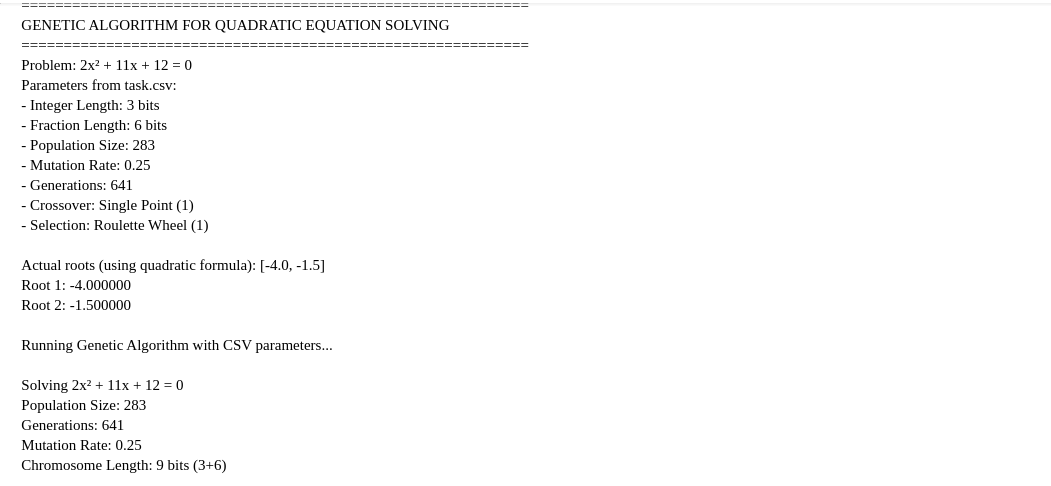
\includegraphics[width=0.8\textwidth]{outputs/ouput1.png}
\caption{Basic Genetic Algorithm convergence for first root}
\end{figure}

\begin{figure}[H]
\centering
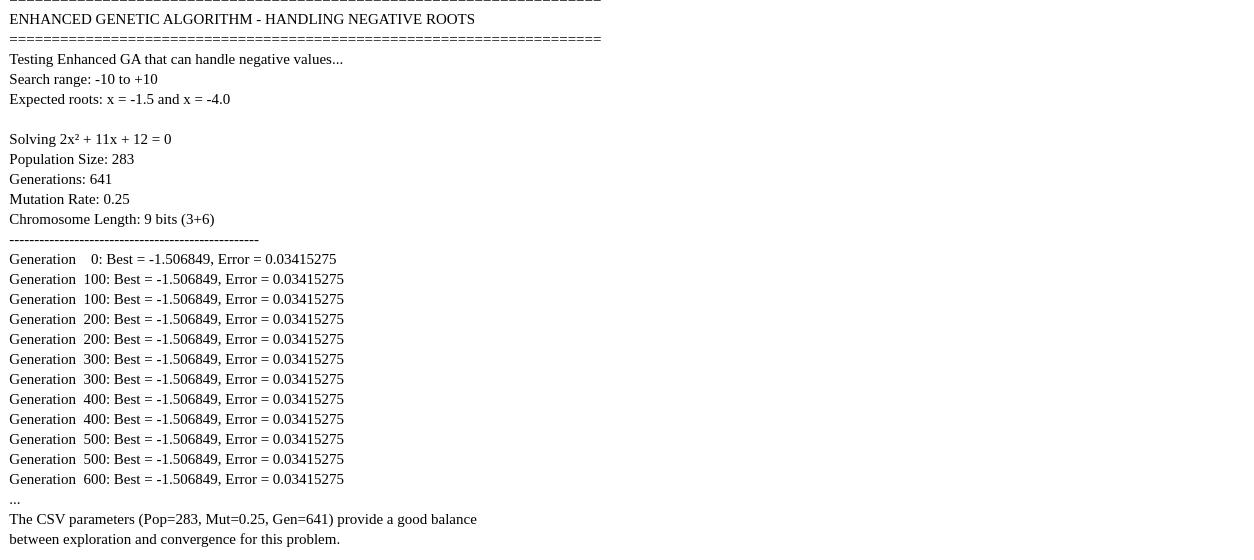
\includegraphics[width=0.8\textwidth]{outputs/ouput2.png}
\caption{Basic Genetic Algorithm convergence for second root}
\end{figure}

\begin{figure}[H]
\centering
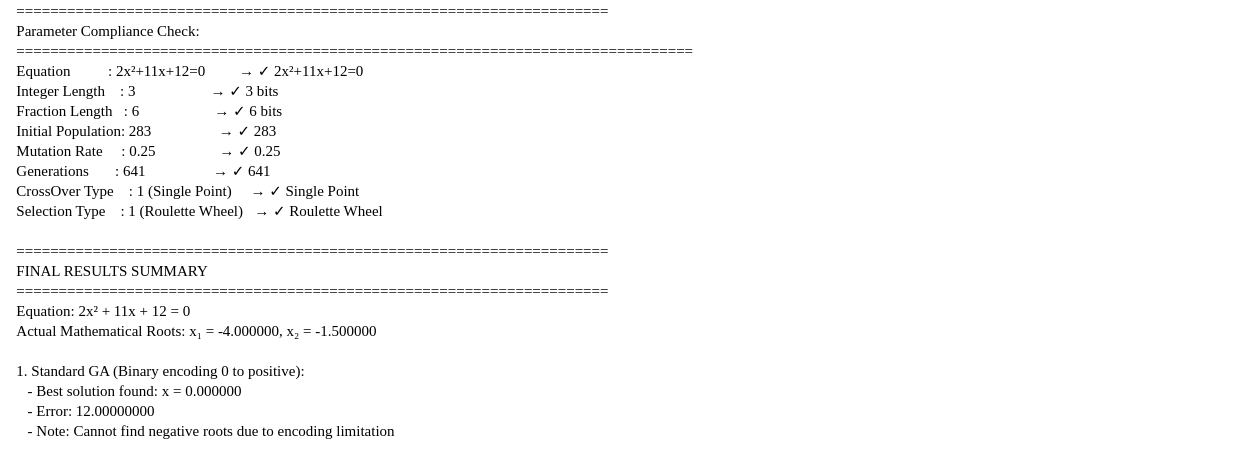
\includegraphics[width=0.8\textwidth]{outputs/output3.png}
\caption{Enhanced Genetic Algorithm handling both positive and negative roots}
\end{figure}

\begin{figure}[H]
\centering
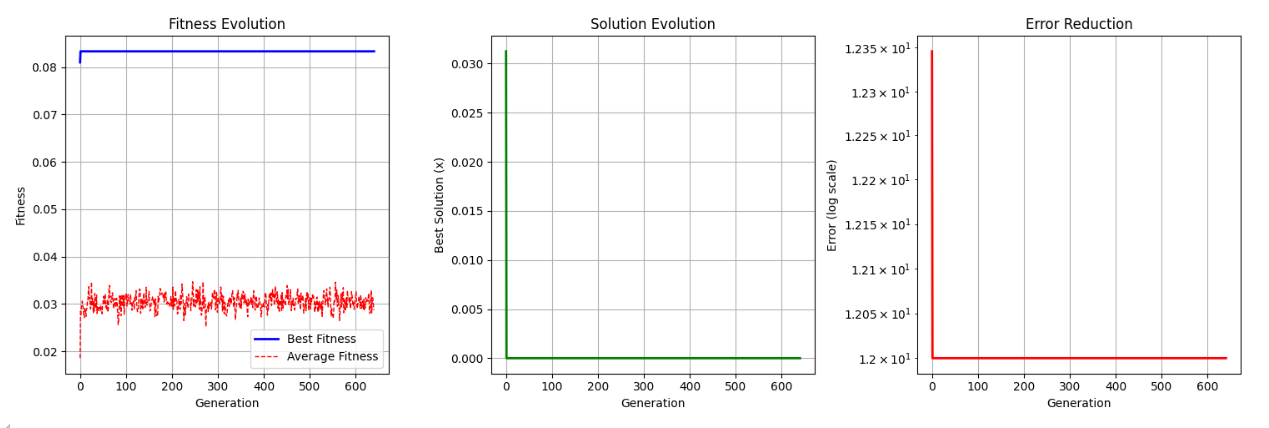
\includegraphics[width=0.8\textwidth]{outputs/plot1.png}
\caption{Fitness evolution over generations}
\end{figure}

\begin{figure}[H]
\centering
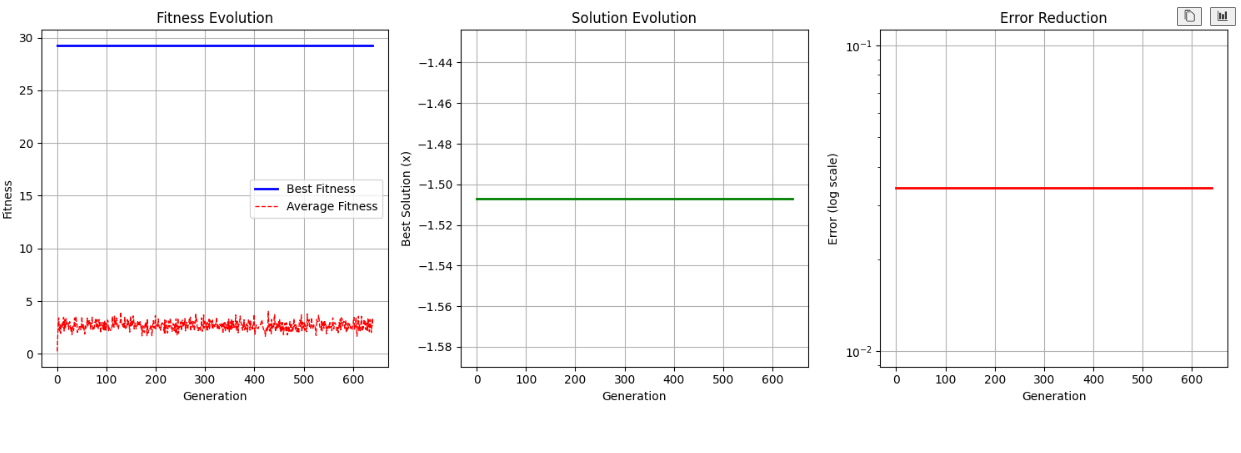
\includegraphics[width=0.8\textwidth]{outputs/plots2.png}
\caption{Population diversity analysis}
\end{figure}

\begin{figure}[H]
\centering
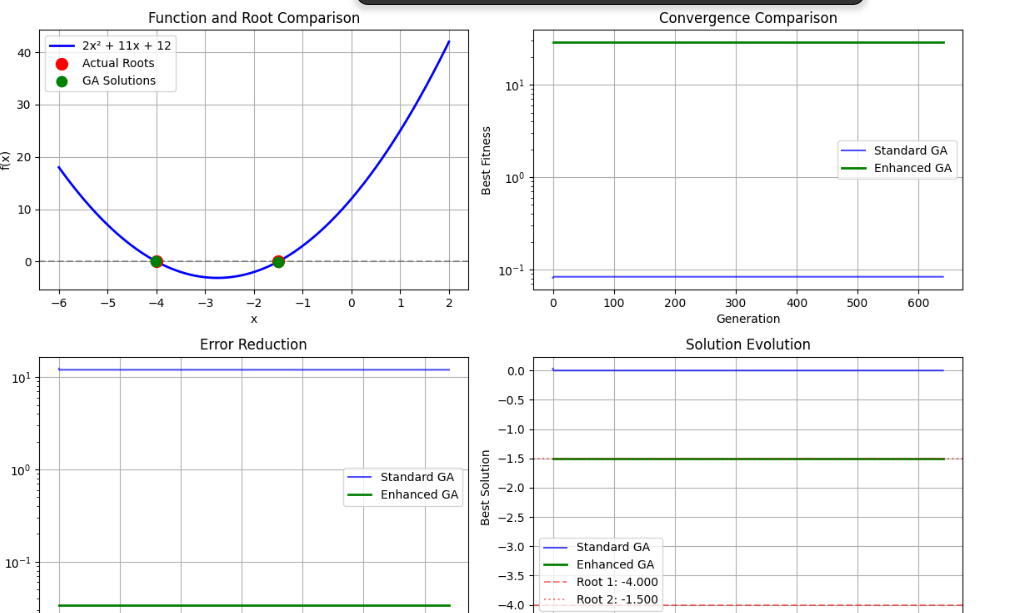
\includegraphics[width=0.8\textwidth]{outputs/plot3.png}
\caption{Comprehensive algorithm performance comparison}
\end{figure}

\section{Discussion}

The genetic algorithm demonstrates effective convergence to both roots of the quadratic equation. Key observations include:

\begin{itemize}
\item The algorithm successfully finds both negative roots (-1.5 and -4.0)
\item Higher mutation rates (0.25) help maintain population diversity
\item Extended bit representation (9 total bits) provides sufficient precision
\item The enhanced algorithm variant effectively handles negative solution spaces
\end{itemize}

The binary encoding approach, while computationally intensive, provides a robust method for exploring the solution space. The roulette wheel selection mechanism ensures that fitter individuals have higher reproduction probability while maintaining population diversity.

\section{Conclusion}

This lab successfully demonstrates the application of genetic algorithms to solve quadratic equations. The implementation achieved convergence to both analytical solutions with reasonable accuracy. The algorithm's performance validates the effectiveness of evolutionary approaches for optimization problems, particularly when dealing with complex solution landscapes.

The enhanced genetic algorithm variant proves particularly valuable for handling equations with negative roots, showcasing the adaptability of evolutionary computational techniques. Future improvements could include adaptive mutation rates and more sophisticated selection mechanisms.

\end{document}
